
\documentclass[a4paper] {report}
\usepackage{geometry}
\usepackage[utf8]{inputenc}
\usepackage[T1]{fontenc}
\usepackage[all]{xy}
\usepackage{textcomp, mathrsfs}
\usepackage{bm}
%\usepackage[french]{babel}
%\frenchbsetup{CompactItemize=false}
\usepackage{xcolor,epic,eepic,multicol, listings}
\usepackage{pstricks, pst-plot, enumitem}
\usepackage{amsmath,amssymb,amsfonts}
\usepackage[framed,amsmath,thmmarks]{ntheorem}
\usepackage{ulem, eurosym}
\usepackage{graphicx, colortbl} 
\usepackage{bmpsize, comment}


\newcommand{\Z}{\mathbb{Z}}
\newcommand{\R}{\mathbb{R}}
\newcommand{\Q}{\mathbb{Q}}
\newcommand{\N}{\mathbb{N}}
\newcommand{\D}{\mathbb{D}}

\theorembodyfont{\upshape} 
\theoremheaderfont{\bfseries}
\theoremseparator{:} 

\newtheorem{defi}{\uline{D�finition}}[section]
\newcommand{\defin}[1]{\begin{defi}\begin{minipage}[t]{16.4}#1\end{minipage}\end{defi}\vspace{0.3cm}}
\newcommand{\defibox}[1]{\fbox{\begin{minipage}{\textwidth}\begin{defi}
\begin{minipage}[t]{16.4cm}#1\end{minipage}\end{defi}\end{minipage}}\vspace{0.3cm}}
\renewcommand{\thedefi}{\empty{}} 

\newtheorem{defis}{\uline{D�finitions}}[section]
\newcommand{\defins}[1]{\begin{defis}\begin{minipage}[t]{16.4}#1\end{minipage}\end{defis}\vspace{0.3cm}}
\newcommand{\defisbox}[1]{\fbox{\begin{minipage}{\textwidth}\begin{defis}
\begin{minipage}[t]{16.4cm}#1\end{minipage}\end{defis}\end{minipage}}\vspace{0.3cm}}
\renewcommand{\thedefis}{\empty{}} 

\newtheorem{theo}{\uline{Th�or�me}}[section]
\newcommand{\theor}[1]{\begin{theo}\begin{minipage}[t]{16.4cm}#1\end{minipage}\end{theo}\vspace{0.3cm}}
\newcommand{\theobox}[1]{\fbox{\begin{minipage}{\textwidth}\begin{theo}
\begin{minipage}[t]{16.4cm}#1\end{minipage}\end{theo}\end{minipage}}\vspace{0.3cm}}
\renewcommand{\thetheo}{\empty{}} 

%\newtheorem{propr}[theo]{\uline{Propri�t�}}
%\newcommand{\propri}[1]{\begin{propr}\begin{minipage}[t]{16.4cm}#1\end{minipage}\end{propr}\vspace{0.3cm}}
%\newcommand{\proprbox}[1]{\fbox{\begin{minipage}{\textwidth}\begin{propr}
%\begin{minipage}[t]{16.4cm}#1\end{minipage}\end{propr}\end{minipage}}\vspace{0.3cm}}
%\renewcommand{\thepropr}{\empty{}} 
%
%\newtheorem{proprs}[theo]{\uline{Propri�t�s}}
%\newcommand{\propris}[1]{\begin{proprs}\begin{minipage}[t]{16.4cm}#1\end{minipage}\end{proprs}\vspace{0.3cm}}
%\newcommand{\proprsbox}[1]{\fbox{\begin{minipage}{\textwidth}\begin{proprs}
%\begin{minipage}[t]{16.4cm}#1\end{minipage}\end{proprs}\end{minipage}}\vspace{0.3cm}}
%\renewcommand{\theproprs}{\empty{}} 

\newtheorem{propo}[theo]{\uline{Proposition}}
\newcommand{\propos}[1]{\begin{propo}\begin{minipage}[t]{16.4cm}#1\end{minipage}\end{propo}\vspace{0.3cm}}
\newcommand{\propobox}[1]{\fbox{\begin{minipage}{\textwidth}\begin{propo}
\begin{minipage}[t]{16.4cm}#1\end{minipage}\end{propo}\end{minipage}}\vspace{0.3cm}}
\renewcommand{\thepropo}{\empty{}} 

\newcommand{\thbox}[2]{\fbox{\begin{minipage}{\textwidth}\textbf{\uline{#1} : }
\begin{minipage}[t]{16.4cm}\upshape{#2}\end{minipage}\end{minipage}}\vspace{0.3cm}}

\newcommand{\sg}[1]{\textbf{\underline{#1}}}
\newcommand{\tsg}[1]{\textbf{\underline{#1} : }}

\renewcommand{\labelenumi}{\textbf{\arabic{enumi})}}
\renewcommand{\labelenumii}{\textbf{\alph{enumii})}}

\newcommand{\rem}[1]{\begin{flushleft}\textbf{\underline{Remarque} : }\begin{minipage}[t]{16.4cm} #1 \end{minipage}\end{flushleft}}
\newcommand{\rems}[1]{\begin{flushleft}\textbf{\underline{Remarques} : }\begin{minipage}[t]{16.4cm} #1 \end{minipage}\end{flushleft}}
\newcommand{\ex}[1]{\begin{flushleft} \textbf{\underline{Exemple} : }\begin{minipage}[t]{16.4cm} #1 \end{minipage} \end{flushleft}}
\newcommand{\exo}[3]{\begin{flushleft}{\bf\LARGE \underline{Exercice #1} : }{\footnotesize #2} {\bf \begin{minipage}[t]{14cm} #3 \end{minipage}} \vspace{0.3cm} 
\\\end{flushleft}}
\newcommand{\titre}[1]{\begin{center} \bf{\huge #1 }\end{center}\vspace{0.5cm}}

\setlength{\unitlength}{1cm}
\psset{arrowinset=0}

\definecolor{string}{rgb}{0.317,0.49,0.345}
%\definecolor{keyword}{rgb}{0.80,0.47,0.2}
%\definecolor{comments1}{rgb}{0,0.6,0}
\definecolor{comments2}{rgb}{0.37,0.55,0.32}
%\definecolor{fonctions}{rgb}{0,0.6,0}
\definecolor{attributs}{rgb}{0.59,0.43,0.56}
\lstset{		language=Python,
 				backgroundcolor=\color{white},
                basicstyle=\color{black}\small,
                keywordstyle=\color{orange}\ttfamily,
                stringstyle=\color{olive}\ttfamily,
                commentstyle=\color{gray}\ttfamily,
                morecomment=[s][\color{lime}]{/**}{**/},
                keepspaces=true,
                morekeywords={module, export, constructor, let, of, number}, 
                showstringspaces=false, 
                tabsize = 2,
                morekeywords={[2]taille, choix, nbIterations, geo, position, links, to, hashNumber, x, y, z}, 
                keywordstyle={[2]\color{attributs}},
                morekeywords={[3]go, goForTheFirstTime, getValue, allKeys, putValue, tan, angleBetweenTwoVectorsBetween0andPi, newFrom, substract, min, max, add, scale, push, setPosition },
                keywordstyle={[3]\color{yellow}}, 
                morekeywords={[4]0, 1, 2, 3, 4, 5, 6, 7, 8, "9"}, 
                keywordstyle={[4]\color{blue}}
}
\newrgbcolor{xdxdff}{0.49019607843137253 0.49019607843137253 1.}
\newrgbcolor{wwzzff}{0.4 0.6 1.}

\renewcommand{\baselinestretch}{1.5}
\begin{document}

\psset{xunit=1cm, yunit=1cm, linewidth=1.1pt, plotpoints=300}
\renewcommand{\labelitemi}{$\bullet$}
\renewcommand{\labelitemii}{$-$}
\setlength{\leftmargini}{0.5cm}
\everymath{\displaystyle}
\graphicspath{{Images/}}

\renewcommand{\thesection}{\Roman{section})}
\renewcommand{\thesubsection}{\Roman{section}.\arabic{subsection})}
\renewcommand{\contentsname}{Sommaire}
\renewcommand{\bibname}{Bibliographie}
\title{UE Projet}
\author{Jonathan GRAFF}
\date{Janvier 2020}
\maketitle
\tableofcontents
\newpage

\section{Introduction}
\subsection{Contexte}

Altran est une entreprise spécialisée dans le conseil, dans l'ingénierie et dans la recherche et développement. Altran accompagne les entreprises du concept à l'industrialisation, pour déve-
lopper de nouveaux produits et services, et intervient depuis plus de 35 ans auprès des grands
acteurs de nombreux secteurs : Automobile, Aéronautique, Spatial, Transport, Energie, Industrie, Communications, Electronique, Logiciel, Internet, Finance, Secteur Public \dots Le groupe est présent dans plus de 30 pays et compte plus de 50000 employés.

Mon projet se situe dans la branche nommée Altran Research. Altran Research est un département recherche interne à la société Altran. Le projet de recherche Sinbad se focalise sur
l'efficacité énergétique dans l'énergie et fait partie du programme Future of Energy, un des sept programmes de recherche du département. Le projet Anagreen est hébergé au sein du projet
Sinbad, c'est une collaboration entre Altran et ArcelorMittal financé par l'Ademe. L'objectif du projet est de développer un outil d'aide à la décision pour la récupération de la chaleur fatale dans l'industrie.

\subsection{Objectifs}

Mon objectif personnel ce semestre, dans le cadre de l'Unité d'Enseignement Projet, est dans un premier temps de m'approprier le sujet, de comprendre les enjeux du problème des réseaux de chaleur, ce domaine m'étant inconnu. Dans un second temps, de me familiariser avec les algorithmes à renforcement profond, afin d'en implémenter un exemple sur un problème-jouet. 

Ce rapport comportera donc une première partie théorique sur le problème des réseaux d'échangeurs de chaleur, de leur utilité, ainsi que des difficultés rencontrées. Dans une deuxième partie, j'expliquerai comment fonctionnent les algorithmes à renforcement profond, et dans une troisième partie, celle-ci pratique, je parlerai de l'implémentation d'un tel algorithme. 

\section{Problèmes des réseaux d'échangeur thermiques}
\subsection{Motivation}

La chaleur fatale est la chaleur résiduelle issue d'un procédé et non utilisée par celui-ci. Une étude de l'ADEME de 2017 \cite{ademe} a montré que cette source d'énergie, si elle n'était pas perdue, représenterait 16\% de la consommation énergétique nationale et représente 36\% de la consommation industrielle. Mais d'après ce rapport, ce nombre est sûrement sous-évalué car ce nombre a été obtenu en ne comptant que les procédés les plus énergivores (comme les fours, séchoirs et chaudières), les rejets les plus accessibles, et les niveaux de température les plus efficaces (au-delà de 100 ° C). Les industries possédant le plus de chaleur fatale sont les industries chimiques, les métaux et matériaux, et l'agro-alimentaire. Il s'agit donc d'un enjeu majeur, aussi bien environnemental qu'économique, que de ne pas gaspiller cette énergie.

Historiquement, jusque dans les années 1970, les entreprises se sont développées au fur et à mesure des années sans se préoccuper de cette source d'énergie perdue, le coût de l'énergie étant particulièrement favorable à l'époque, mais aussi la préoccupation écologique et notamment du réchauffement climatique étant alors très faible. Aujourd'hui, il y a une prise de conscience plus importante de ce sujet, l'énergie est plus chère qu'auparavant, il y a des taxes sur les rejets polluants, et des fonds d'aide sont alloués aux entreprises souhaitant investir dans ce domaine. Pour toutes ces raisons, les entreprises se sont donc progressivement intéressées à l'importance de la récupération de la chaleur fatale.

Des années de développement interne sans tenir compte de ce problème font qu'aujourd'hui
il est très difficile de revenir en arrière sur ce sujet, la configuration des complexes industriels ne s'y prêtant pas toujours. De plus, de nouvelles installations nécessiteraient parfois des coupures dans les chaînes de production, ce qui pour certaines compagnies n'est tout simplement pas envisageable, car synonyme de perte de chiffre d'affaires trop importante.

C'est dans ce contexte qu'Anagreen propose de développer un outil d'aide à la décision pour la récupération de la chaleur fatale. L'outil propose une méthodologie qui permet de recycler la chaleur interne d'un procédé pour réduire sa demande en énergie externe. Dans un premier temps, la méthodologie permet d'identifier les gisements de chaleur disponible, puis dans un deuxième temps de construire un réseau d'échangeurs pour permettre le transfert de chaleur entre flux chauds et flux froids.

\subsection{Généralités sur les échangeurs thermiques}
Afin de récupérer de la chaleur fatale pour une utilisation en interne, il est nécessaire de
placer des échangeurs thermiques entre les flux chauds, ceux nécessitant d'être refroidis, et les flux froids, ceux nécessitant d'être réchauffés.
Un échangeur thermique est un dispositif permettant de transférer de la chaleur d'un flux chaud vers un flux plus froid, sans les mélanger. Même si cela ne rentre pas directement dans le cadre du rapport, il est intéressant de comprendre quelques bases sur les échangeurs.

\subsubsection{Types d'échangeurs}
Il existe trois principaux modes de transfert de chaleur : 
\begin{itemize}
\item à co-courant : les deux flux ont la même direction, dans ce cas le flux froid aura nécessairement en sortie une température moins élevée que celle du flux chaud. La figure \ref{evo1} représente le profil de l'évolution des températures des flux en fonction de la surface d'échange. 

\begin{figure}[!h]
\centering
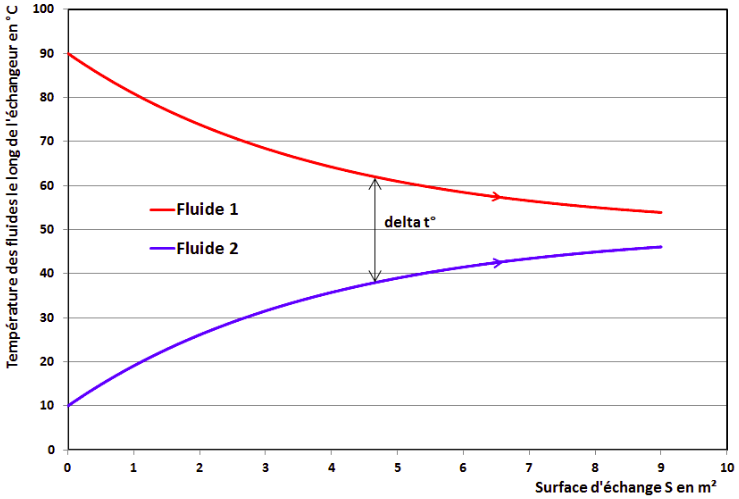
\includegraphics[scale=0.3]{1.png}
\caption{Evolution des températures des flux lors d'un transfert à co-courant}
\label{evo1}
\end{figure}

\item à contre-courant : les flux circulent parallèlement mais dans des sens opposés, dans ce cas, le flux froid peut avoir une température de sortie supérieure à elle du flux chaud. En général, ces échangeurs sont plus efficaces. La figure \ref{evo2} montre le profil de l'évolution des températures en fonction de la surface d'échange dans ce cas : 

\begin{figure}[!h]
\centering
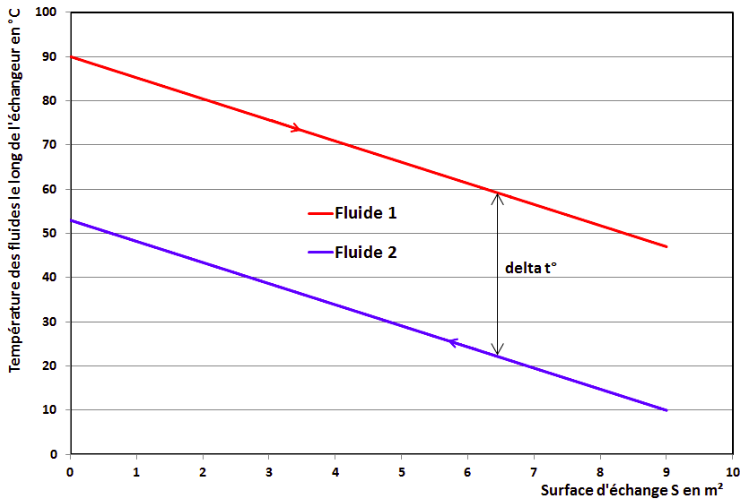
\includegraphics[scale=0.27]{2.png}
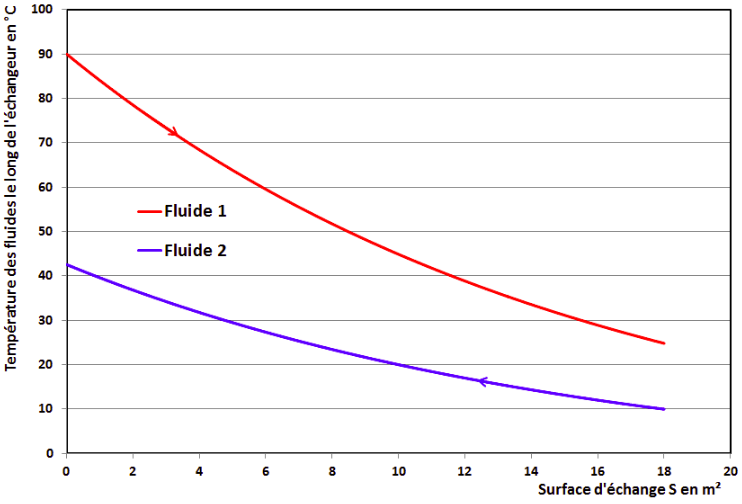
\includegraphics[scale=0.27]{3.png}
\caption{Evolution des températures des flux lors d'un transfert à contre-courant}
\label{evo2}
\end{figure}

\item à courant croisés : les deux flux ont des directions perpendiculaires.
\end{itemize}

Il existe différents types d'échangeurs : à tube, à faisceau tubulaire, à spirales, à plaques, à baïonnettes, à ailettes..., et pour chacun différentes tailles et surfaces d'échange.

Chaque échangeur a également un coût différent, lié à sa surface d'échange, et donc à sa performance. Le problème du dimensionnement des échangeurs est un sujet de recherche en soi dont nous ne nous préoccuperons pas ici. 

\subsubsection{Montage des échangeurs}

Ces échangeurs peuvent être montés de quatre façons différentes : 
\begin{itemize}
\item en série : 

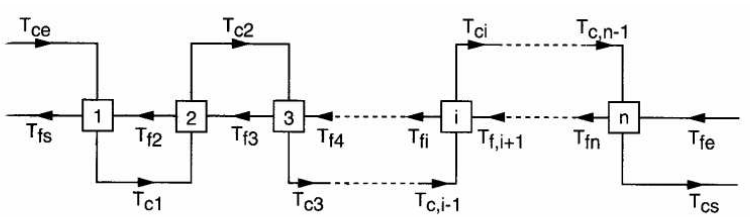
\includegraphics[scale=0.5]{4.png}

\item un en parallèle et l'autre en série : 

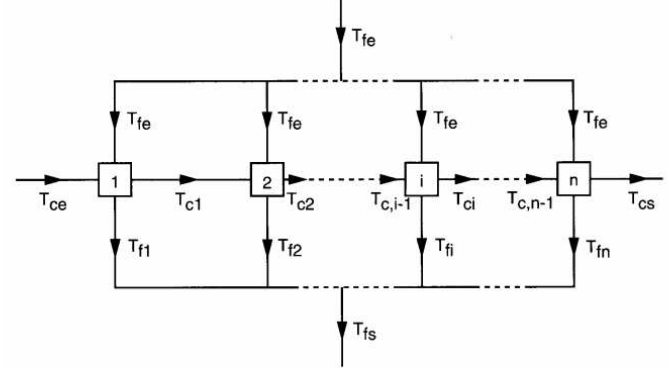
\includegraphics[scale=0.5]{5.png}

\item les deux en parallèles. Cette méthode est moins utilisée que les autres pour des raisons de performances moindres.

\item en maillage : 

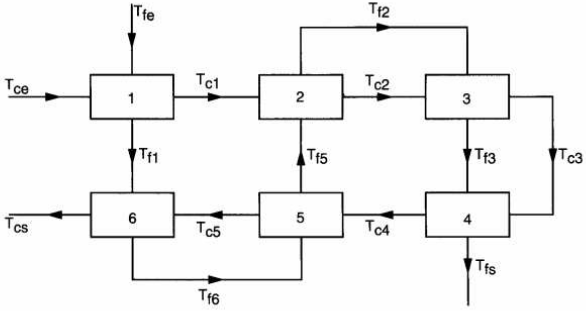
\includegraphics[scale=0.5]{6.png}

\end{itemize}


\subsection{Réseaux d'échangeurs thermiques}

Une entreprise possédant en général plusieurs flux chauds et plusieurs flux froids, il faudrait don placer plusieurs échangeurs thermiques afin d'optimiser le rendement énergétique. Toute la question est de savoir quels échangeurs placer (problèmes de coût et de maintenance), où les
placer (endroits accessibles et optimaux), et quand les placer (l'installation pouvant nécessiter
un arrêt des machines, celui-ci n'étant en général pas souhaitable).

Ce problème d'apparence simple est en fait un problème combinatoire des plus complexes. Il s'agit en fait, comme l'ont montré Furman et Sahinidis \cite{NP}, d'un problème NP-difficile, c'est-à-dire que le nombre d'opérations pour résoudre ce problème croit exponentiellement en fonction du nombre de paramètres d'entrée, mais que même la vérification d'une solution est un problème de complexité exponentielle.

A titre d'exemple, supposons qu'on ait 10 flux chauds, et 10 flux froids, et qu'on souhaite placer au maximum 15 échangeurs thermiques dans notre réseau. Le premier échangeur a donc $10 \times 10 = 100$ possibilités pour être placé. Le deuxième a $11 \times 11 = 121$ possibilités pour être placé, car chaque flux sur lequel on a placé le premier échangeur est divisé en deux parties,
une avant l'échangeur, l'autre après. En continuant ainsi, et en divisant à la fin par $15!$ pour ne pas compter les permutations des échangeurs comme une autre solution, on trouve à l'aide d'un
algorithme, qu'il y a de l'ordre de $2.295 \times 10^{24}$ solutions possibles. Bien sûr, tout ceci sans tenir
compte d'autres paramètres, comme le type d'échangeurs, leur surface...

\subsection{Etat de l'art}

Pour essayer de s'approcher de la solution optimale à ce problème, plusieurs méthodes sont aujourd'hui utilisées :
\begin{itemize}
\item Tout d'abord il y a la méthode empirique, s'appuyant sur des avis d'experts pour déterminer une solution. Cette méthode ne prend souvent pas le problème dans son ensemble, et même si cette solution est souvent satisfaisante, elle ne garantit pas d'être optimale.
\item La méthode du pincement, consiste à diviser le problème en deux sous-problèmes plus simples.
Elle repose sur des principes thermodynamiques, est utilisée depuis plus de 30 ans et fait encore aujourd'hui l'objet de nombreuses études. Elle fournit en général de meilleurs résultats que la méthode empirique, mais ne trouve pas non plus nécessairement l'optimum global.
\item Enfin, d'autres méthodes plus récentes, consistent à trouver des algorithmes mathématiques pour résoudre le problème. Parmi ces problèmes, on peut citer les algorithmes gloutons, des algorithmes de programmation linéaire ou non-linéaire mixte entière (MILP ou MINLP), des algorithmes génétiques, des méthodes stochastiques, de recuit simulé...
\end{itemize} 

\section{Proposition d'une nouvelle solution : l'apprentissage par renforcement profond}

L'objectif du projet est de vérifier si une méthode utilisant les algorithmes d'apprentissage par réseaux de neurones à renforcement profond, pourrait résoudre le problème d'optimisation combinatoire.

Dans un article, l'équipe de Google Brain \cite{google} a obtenu des résultats intéressants sur le problème combinatoire du trajet à suivre par le voyageur de commerce et l'objectif du projet Anagreen est de se demander si ces mêmes résultats pourraient être transposables sur ce problème de réseaux d'échangeurs de chaleur. 

Dans le cadre de ce projet tutoré, nous allons détailler comment fonctionne ce type d'apprentissage et nous allons voir son fonctionnement sur des exemples simples.


\subsection{Apprentissage par renforcement}

L'apprentissage par renforcement est un procédé d'apprentissage où un agent (un robot par exemple) apprend par lui-même le comportement à adopter face à un problème pour le résoudre. L'agent est placé dans un environnement et peut avoir plusieurs états. Par rapport à chaque état, il peut effectuer un ensemble d'actions. 

\begin{figure}[!h]
\centering
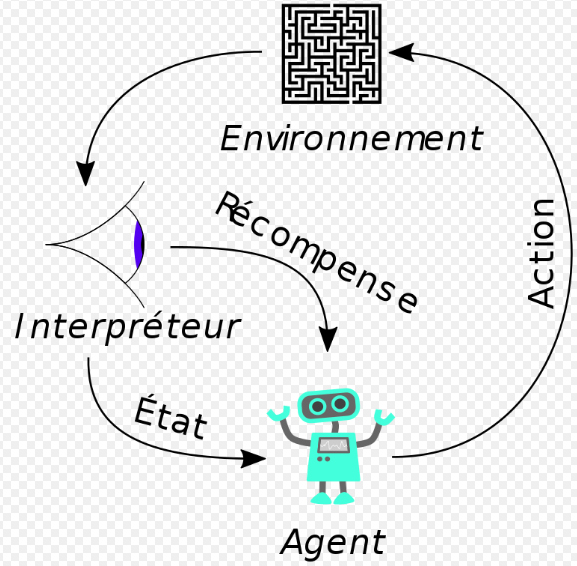
\includegraphics[scale=0.3]{7.png}
\caption{Schéma représentant l'apprentissage par renforcement}
\label{renf}
\end{figure}

L'action ou les probabilités d'effectuer chaque action selon l'état dans lequel l'agent se trouve est une fonction appelée la politique. 
A chaque action effectuée l'agent va recevoir une "récompense", modélisée sous la forme d'un nombre réel, positif ou nul. Pendant la phase d'apprentissage, l'agent va alterner entre deux comportements :

\begin{itemize}
\item une phase d'exploration où l'agent va tester aléatoirement de nouvelles actions, afin de voir si celles-ci sont bonnes ou mauvaises, et actualiser sa politique en fonction.
\item une phase d'exploitation, où la politique actuelle est éprouvée.
\end{itemize}

L'agent alterne entre ces deux comportements aléatoirement, et au cours de l'apprentissage, la probabilité d'exploration est en général diminuée au fur et à mesure que la politique s'approche de la politique optimale.

Il existe plusieurs variations pour ces types d'algorithmes à renforcement : basé sur un modèle ou non, à différence temporelle, Q-learning, méthodes acteurs-critiques...

\subsection{Modélisation mathématique}
\subsubsection{Notations}

On note $S=\lbrace s_i \rbrace_{i \in I} $ l'ensemble des états dans lequel l'agent peut se trouver, et $A_s = \lbrace a_i \rbrace_{i \in I_s} $ l'ensemble des actions possibles en se trouvant à l'état $s$. On note $A = \cup_{s \in S} A_s$ l'ensemble des actions possibles. Un état est dit \textbf{terminal} si l'expérience se termine à ce moment-là (par exemple perdre ou gagner un jeu...).

L'environnement renvoie à l'agent, en fonction de son état $s$ et de son action $a$, un autre état $s'$ et une récompense $r$, qui est un nombre réel. Mathématiquement, $env$ est une fonction $$env :\begin{array}[t]{lcr}
S\times A &\rightarrow& S \times \R\\
(s,a) & \mapsto & (s', r)\\\end{array}$$

Dans le cas d'un environnement stochastique, celui-ci ne renvoie pas directement un nouvel état, mais un vecteur de probabilités d'aller dans chaque état. 

Le but est de trouver une suite de paires état-action $(s,a)$ qui maximise la récompense $G$, où $G$ vérifie :
$$G = \sum_{t} \gamma ^t r_t$$
Si l'environnement est stochastique, on veut alors maximiser le nombre $E(G)$.


$\gamma$ est le \textbf{facteur de réduction}, c'est un réel de $[0,1]$. Il sert à pondérer les récompenses selon le moment où elles sont reçues : 

\begin{itemize}
\item si $\gamma=0$, seule la récompense immédiate compte. Ce n'est pas un cas intéressant, puisque l'agent ne prendra jamais le risque d'aller voir dans un autre état, moins intéressant à court terme, mais peut-être plus à long terme. 
\item si $\gamma=1$, toutes les récompenses valent la même chose, peu importe le temps où elles sont reçues. Ce n'est pas très intéressant, puisque si le jeu peut être infini, la récompense sera infinie.
\item pour $\gamma$ dans $]0,1[$, la somme converge. Plus $\gamma$ est proche de $1$, plus le gain à long terme est intéressant. En pratique, on prend en général $\gamma$ entre $0.9$ et $1$ exclu.
\end{itemize}

On note : 
$$
Q^{*}(s,a) := \max_{ (s_t,a_t)\ _{t\geq 0}}\left( \sum_{t\geq 0} \gamma^t r_t  \ \big | s_0=s,a_0=a\right)
$$

La fonction $Q^{*}$ est appelée la $Q$-fonction optimale. Il s'agit de la fonction qui renvoie la récompense maximale pouvant être obtenue à partir d'un état et d'une action de départ. Evidemment, cette fonction n'est en général pas connue. On va chercher à l'approcher, car une fois cette fonction connue, on connaitra aussi la trajectoire à suivre pour obtenir ce maximum :

$$
a_1 = \text{argmax}_{a\in A_{s_1}} Q^{*}(s_1,a), ~ a_2 = \text{argmax}_{a\in A_{s_2}} Q^{*}(s_2,a) \text{ etc}.
$$

On définit également à partir de $Q$ et $Q^*$ les fonctions de valeur $V$ et $V^*$ par : 

$$V(s)=\max_{a\in A} Q(s,a)\text{ et }V^*(s)=\max_{a\in A} Q^*(s,a)$$

Cette fonction représente la valeur maximale pouvant être atteinte en se trouvant à l'état $s$.  Dans l'algorithme du $Q$-learning, on va chercher à approximer $Q^*$ directement. Dans celui du $V-$learning, on va plutôt approximer $V$.


\subsubsection{Théorème de Bellmann}

Soient $(s,a)$ un couple état-action, et posons $(s',r)= env(s,a)$.  La fonction $Q^{*}$ vérifie:   
$$
Q^{*}(s,a) = r + \gamma \max_{a'\in A_{s'}} Q^{*}(s',a')
$$

Ce théorème va nous permettre d'approcher la fonction $Q^*$ au moyen d'un algorithme itératif. En effet, si une fonction $Q$ vérifie "à peu près" la relation précédente, alors $Q$ sera proche de $Q^*$. 

\subsubsection{Algorithme du $Q$-learning}

En pratique : \begin{enumerate}

\item on initialise $Q$ à $0$, $\epsilon$ à $1$

\item on choisit un état $s$ aléatoirement

\item on choisit une action $a$ selon le principe suivant : on choisit aléatoirement une action avec une probabilité de $\epsilon$ : c'est la phase d'\textbf{exploration}. Et avec une probabilité de $1-\epsilon$, on choisit l'action qui maximise $Q(s,a)$ (avec le $Q$ courant) : c'est la phase d'\textbf{exploitation}.

\item on calcule $s', r = env(s, a)$ et on met à jour : $$ 
Q(s,a) = r + \gamma \max_{a'} Q(s',a')
$$

\item on diminue $\epsilon$.

\item si l'état $s$ n'est pas terminal, on recommence à l'étape 3 avec $s=s'$. S'il l'est, on recommence à l'étape 2. 

\item On arrête l'algorithme selon un critère d'arrêt, par exemple au bout d'un nombre fixé d'itérations

\end{enumerate} 

\subsection{Apprentissage par renforcement profond}

Le problème de la méthode ci-dessus est que le nombre d'états est en général immense, souvent même infini. Il est alors impossible de construire la fonction $Q$ de façon à ce que tous les couples états-actions soient pris en compte. On utilise alors à la place un réseaux de neurones pour pouvoir prédire la valeur de la fonction $Q$, en général un réseau de neurones à plusieurs couches cachées, d'où le nom "profond".

En pratique, on choisit une taille de batch, on initialise les poids $\omega$ de notre réseau de neurones, on part d'un couple état-action initial $(s,a)$, et on construit un batch d'états-action en suivant la même stratégie que précédemment, selon $\epsilon$. 

Une fois ce batch construit, on l'utilise pour modifier les poids $\omega$ du réseau de façon à ce que la distance entre les $
Q(s,a) \text{ et les } r + \gamma \max_{a'} Q(s',a')$ soit minimale (où $s'$ est l'état renvoyé après l'action $a$).

Dans le cadre du projet tutoré, nous allons nous concentrer sur l'apprentissage par renforcement standard. 

\section{Implémentation d'un exemple}

Dans cette partie, l'objectif est d'illsustrer le fonctionnement de l'algorithme du Q-learning vu plus tôt. Nous allons donc voir les performances de l'entraînement auprès d'un agent. L'environnement, et le programme sont inspirés de \cite{gridW}.

\subsubsection*{L'environnement}

Comme environnement, nous allons prendre une grille dans laquelle nous allons placer l'agent dans la case en-haut à gauche. Dans la case du bas à droite, on y place un "trésor" et dans celle juste au-dessus, une "bombe". 

Le but du jeu est pour l'agent de se déplacer selon quatre directions (haut, bas, gauche, ou droite) pour aller chercher le trésor, en évitant bien sûr la bombe, et ceci le plus vite possible. Certaines cases seront des obstacles. S'il se trouve sur un bord de la grille, et que la direction choisie est vers l'extérieur de la grille, l'agent restera sur place.

Les états terminaux sont donc les deux cases "bombe" et "trésor". 

\begin{figure}[!h]
\centering
$$\begin{array}{|c|c|c|c|c|}
\hline
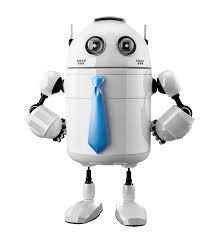
\includegraphics[scale=0.15]{agent.jpeg} & \hspace*{1cm} &  \hspace*{1cm}&  \hspace*{1cm} & \\
\hline
& & \cellcolor{black} & & \\
& & \cellcolor{black} & & \\
\hline
& \cellcolor{black} & & & 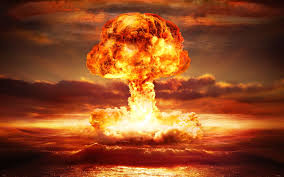
\includegraphics[scale=0.15]{bombe.jpeg}\\
\hline
& & & & 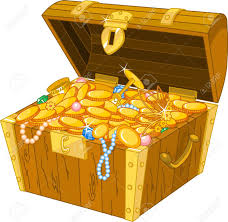
\includegraphics[scale=0.15]{tresor.jpeg} \\
\hline
\end{array}
$$
\caption{L'environnement GridWorld pour une grille $4 \times 5 $ avec deux obstacles}
\label{gridw}
\end{figure}

\newpage
\subsubsection*{La récompense}

Pour l'entraînement, l'agent recevra les récompenses suivantes : 

\begin{itemize}
\item +10 pour un déplacement sur le trésor
\item -10 pour un déplacement sur la bombe
\item -1 pour chaque déplacement
\end{itemize}

Voici une figure représentant les récompenses pouvant être gagnées : \medskip
\begin{figure}[!h]
\centering
$$\begin{array}{|c|c|c|c|c|}
\hline
-1 & -1 & -1 & -1 & -1 \\
\hline
-1 & -1 & 0 & -1 & -1 \\
\hline
-1 & 0 & -1 & -1 & -10 \\
\hline
-1 & -1 & -1 & -1 & 10 \\
\hline
\end{array}
$$

\caption{Les récompenses obtenues dans Gridworld}
\label{recomp}
\end{figure}


\subsubsection*{Les résultats}

Le programme a donc tourné deux fois, une fois avec un agent qui ne choisit son chemin qu'aléatoirement, et une autre fois avec un agent qui apprend.

Voici les récompenses obtenues par ces deux agents sur 500 essais : 

\begin{figure}[!ht]
\hspace*{0cm}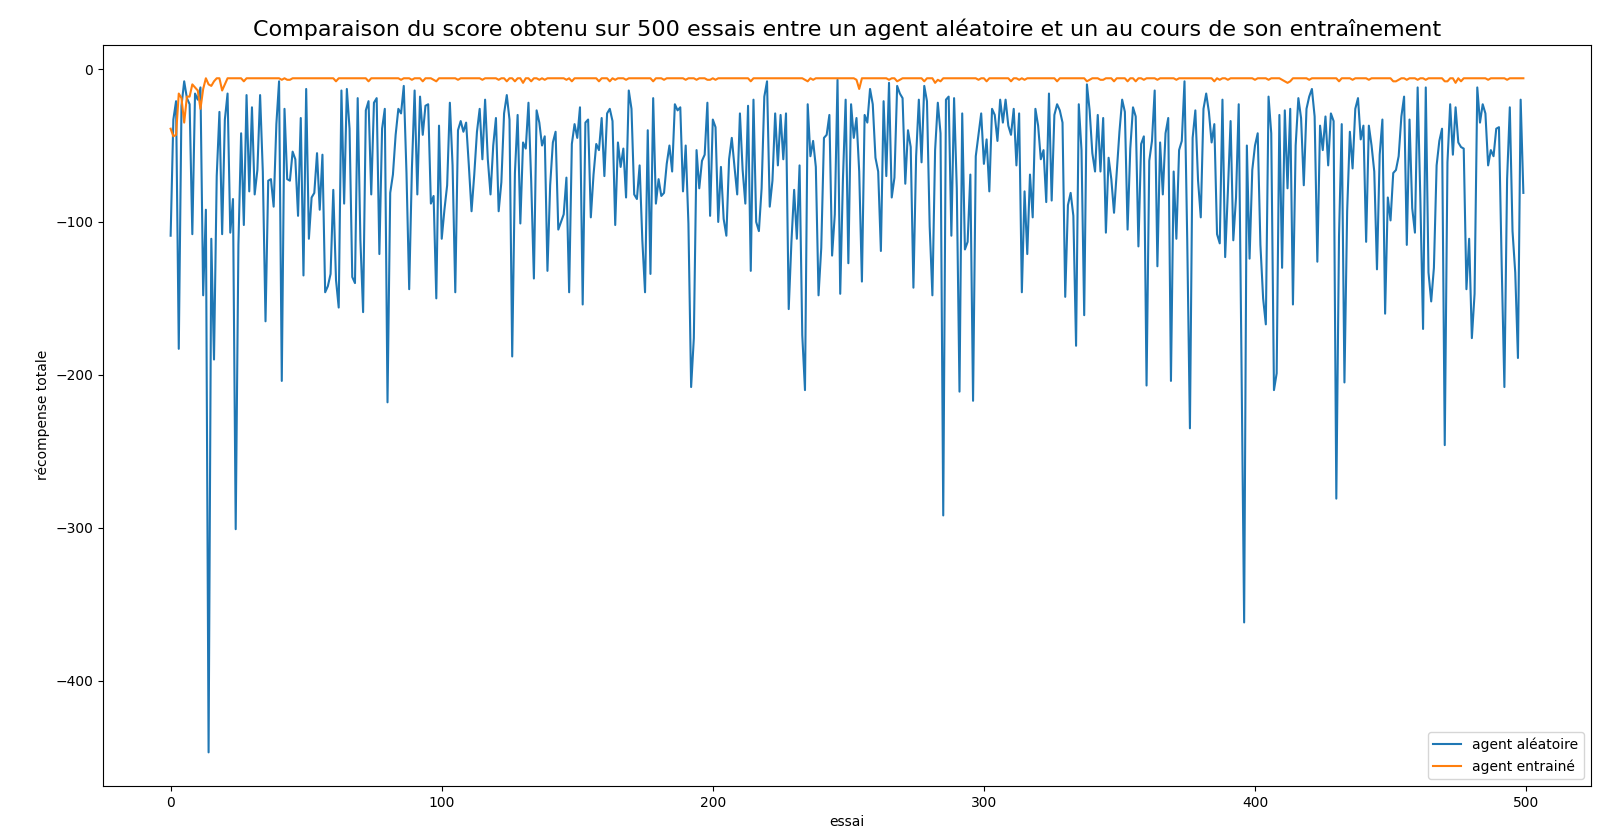
\includegraphics[scale=0.26]{resultats.png}
\caption{Comparaison des récompenses}
\label{recompgraph}
\end{figure}

On remarque que l'agent qui apprend est très vite beaucoup plus efficace que l'agent aléatoire qui lui peut prendre des valeurs jusqu'à $-500$. Le programme fonctionne donc bien. En regardant les résultats de l'agent entraîné : 

\begin{figure}[!ht]
\hspace*{0cm}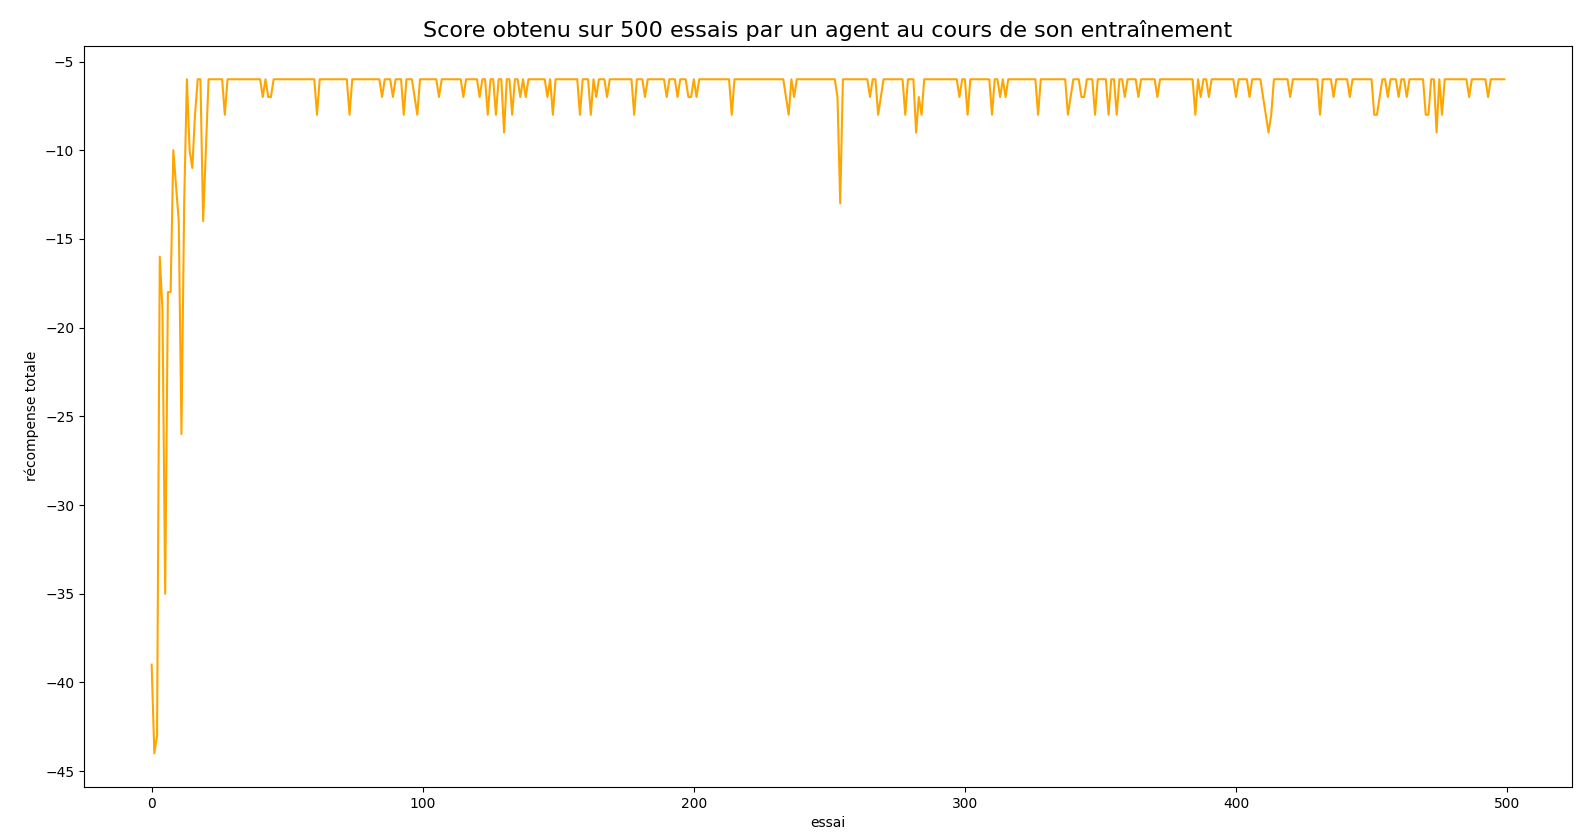
\includegraphics[scale=0.26]{resultats2.png}
\caption{Récompenses de l'agent au cours de son entraînement}
\label{recompgraph2}
\end{figure}

On voit bien que les résultats varient beaucoup au début, puis de moins en moins au fur et à mesure de l'apprentissage de l'agent. 

\subsubsection*{La Q-table}

La Q-table est composée, pour chaque case de la grille, d'un dictionnaire. Ses quatre clés sont les quatre actions (haut, gauche, droite et bas) et ses valeurs sont celles de $Q(etat, action)$. Au début, toutes ses valeurs sont égales à 1. Voici sur un exemple $3\times 3$, comment, à l'aide de la formule de Bellmann la Q-table est actualisée. Le A rouge représente la position de l'agent, le B et le T la bombe et le trésor.

\begin{figure}[!ht]
\centering
$$\begin{array}{|c|c|c|}
\hline
0                      & 0                           & 0 \\
0\hspace*{0.25cm}\textcolor{red}{A}\hspace*{0.25cm} 0 & 0\hspace*{0.8cm} 0                  & 0\hspace*{0.6cm}0 \\
0          & 0          & 0 \\
\hline
0          & 0                            & 0 \\
0\hspace*{0.6cm}0   & 0\hspace*{0.6cm} 0                  & 0\hspace*{0.25cm}\textcolor{red}{B}\hspace*{0.25cm} 0 \\
0           & 0          & 0 \\
\hline
0          & 0                         & 0\\
0\hspace*{0.6cm} 0                     & 0\hspace*{0.6cm}0                & 0\hspace*{0.25cm}\textcolor{red}{T}\hspace*{0.25cm} 0 \\
0                            & 0        & 0 \\
\hline
\end{array}
$$
\caption{La Q-table au début}
\end{figure}

Au début, l'agent est dans une phase d'exploration. Il choisit au hasard une direction. Imaginons qu'il choisisse d'aller à droite. Il recevra une récompense de $-1$. Donc : 
$$Q((0,0), "droite") = -1 + \max_{a'} Q((0,1), a') = -1+0 = -1$$

Supposons qu'ensuite, il aille à nouveau droite, le même calcul nous donne : 
$$Q((0,1), "droite") = -1$$

Si à l'étape suivante, il choisit d'aller vers le bas, alors la récompense sera de $-10$, et donc : $$Q((0,2), "bas") = -10 + \max_{a'} Q((0,1), a') = -10+0 = -10$$

A la fin du premier épisode, on aura donc : 
\begin{figure}[!ht]
\centering
$$\begin{array}{|c|c|c|}
\hline
0                      & 0                           & 0 \\
0 -1 & 0 \hspace*{0.6cm} -1 & 0\hspace*{0.6cm}0 \\
0          & 0          & -10 \\
\hline
0          & 0                            & 0 \\
0\hspace*{0.6cm}0   & 0\hspace*{0.6cm} 0                  & 0\hspace*{0.25cm}\textcolor{red}{B A}\hspace*{0.25cm} 0 \\
0           & 0          & 0 \\
\hline
0          & 0                         & 0\\
0\hspace*{0.6cm} 0                     & 0\hspace*{0.6cm}0                & 0\hspace*{0.25cm}\textcolor{red}{T}\hspace*{0.25cm} 0 \\
0                            & 0        & 0 \\
\hline
\end{array}
$$
\caption{La Q-table à la fin du premier épisode}
\end{figure}

Imaginons un deuxième épisode où le chemin choisi sera "droite bas bas droite". 
Alors $Q((0,0), "droite")=-1$, $Q((0,1), "bas")=-1$, $Q((1,1), "bas")=-1$ et $Q((2,1), "droite")=10$.

A la fin du deuxième épisode, on aura donc : 
\begin{figure}[!ht]
\centering
$$\begin{array}{|c|c|c|}
\hline
0                      & 0                           & 0 \\
0 -1 & 0 \hspace*{0.6cm} -1 & 0\hspace*{0.6cm}0 \\
0          & -1          & -10 \\
\hline
0          & 0                            & 0 \\
0\hspace*{0.6cm}0   & 0\hspace*{0.6cm} 0                  & 0\hspace*{0.25cm}\textcolor{red}{B}\hspace*{0.25cm} 0 \\
0           & -1          & 0 \\
\hline
0          & 0                         & 0\\
0\hspace*{0.6cm} 0                     & 0\hspace*{0.6cm}10                & 0\hspace*{0.25cm}\textcolor{red}{T A}\hspace*{0.25cm} 0 \\
0                            & 0        & 0 \\
\hline
\end{array}
$$
\caption{La Q-table à la fin du deuxième épisode}
\end{figure}

Si à un troisième épisode, le chemin choisi est "bas droite bas droite". 
Alors $Q((0,0), "bas")=-1$, $Q((1,0), "droite")=-1$, $Q((1,1), "bas")=-1+10=9$ et $Q((2,1), "droite")=10$.

A la fin du troisième épisode, on aura donc : 
\begin{figure}[!ht]
\centering
$$\begin{array}{|c|c|c|}
\hline
0                      & 0                           & 0 \\
0 -1 & 0 \hspace*{0.6cm} -1 & 0\hspace*{0.6cm}0 \\
-1          & -1          & -10 \\
\hline
0          & 0                            & 0 \\
0\hspace*{0.6cm}-1   & 0\hspace*{0.6cm} 0                  & 0\hspace*{0.25cm}\textcolor{red}{B}\hspace*{0.25cm} 0 \\
0           & 9         & 0 \\
\hline
0          & 0                         & 0\\
0\hspace*{0.6cm} 0                     & 0\hspace*{0.6cm}10                & 0\hspace*{0.25cm}\textcolor{red}{T A}\hspace*{0.25cm} 0 \\
0                            & 0        & 0 \\
\hline
\end{array}
$$
\caption{La Q-table à la fin du troisième épisode}
\end{figure}
\newpage
Avec deux autres épisodes on obtiendra donc la Q-table suivante : 

\begin{figure}[!ht]
\centering
$$\begin{array}{|c|c|c|}
\hline
0                      & 0                           & 0 \\
0 -1 & 0 \hspace*{0.6cm} -1 & 0\hspace*{0.6cm}0 \\
7          & -1          & -10 \\
\hline
0          & 0                            & 0 \\
0\hspace*{0.6cm}8   & 0\hspace*{0.6cm} 0                  & 0\hspace*{0.25cm}\textcolor{red}{B}\hspace*{0.25cm} 0 \\
0           & 9         & 0 \\
\hline
0          & 0                         & 0\\
0\hspace*{0.6cm} 0                     & 0\hspace*{0.6cm}10                & 0\hspace*{0.25cm}\textcolor{red}{T A}\hspace*{0.25cm} 0 \\
0                            & 0        & 0 \\
\hline
\end{array}
$$
\caption{La Q-table à la fin du cinquième épisode}
\end{figure}



Voici la Q-table de l'agent entraîné à la fin de son apprentissage, avec des valeurs arrondies à $10^{-2}$. En rouge est notée la valeur maximale : 
\begin{figure}[!ht]
\centering
$$\begin{array}{|c|c|c|c|c|}
\hline
-2.02                           & 0.60                          & 2.11                           & 1.41                           & -0.8 \\
-1.07~ ~ \textcolor{red}{4.00}  & 0.55~ ~ \textcolor{red}{5.00} & -0.57~ ~ \textcolor{red}{6.00} & 1.71~ ~ -1.21                  & -0.80~ ~ -0.80 \\
-3.30                           & -2.59                         & 0.60                           & \textcolor{red}{7.00}          & \textcolor{red}{-0.10} \\
\hline
-2.56                         & \textcolor{red}{1.29}        & 0.00           & 4.07                            & -0.46 \\
-2.60~ ~ -2.54                & 2.51~ ~-2.57                 & 0.00~ ~ 0.00   & 6.46~ ~ -0.40                   & \textcolor{red}{3.46}~ ~ -0.50 \\
\textcolor{red}{-2.48}        & -2.58                        & 0.00           & \textcolor{red}{8.00}          & -0.47 \\
\hline
-1.78                          & 0.00          & -0.10          & 1.56                         & 0.00\\
-1.80~ ~ -1.80                 & 0.00~ ~ 0.00  & 0.04~ ~ \textcolor{red}{5.14}                     & 1.35~ ~ -4.69                & 0.00~ ~ 0.00 \\
\textcolor{red}{-1.20}         & 0.00          & -0.10                            & \textcolor{red}{9.00}        & 0.00 \\
\hline
-1.20                              & -0.59                          & -0.10                           &  6.28                           & 0.00 \\
-1.12~ ~ \textcolor{red}{1.03}     & -0.56~ ~ \textcolor{red}{4.31} & -0.34~ ~ \textcolor{red}{8.13}  &  2.25~ ~ \textcolor{red}{10.00} & 0.00~ ~ 0.00 \\
-1.10                              & -0.60                          & -0.10                           & 4.70                           & 0.00 \\
\hline
\end{array}
$$
\caption{La Q-table de l'agent à la fin}
\end{figure}
\newpage
On voit bien que la valeur maximale dirige bien vers le bon chemin. Si le chemin ne varie pas (si $\epsilon=0$ par exemple), le chemin choisi sera donc le suivant : 

\begin{figure}[!h]
\centering
$$\begin{array}{|c|c|c|c|c|}
\hline
\rightarrow & \rightarrow & \rightarrow & \downarrow & \\
\hline
  &  & \cellcolor{black} & \downarrow &  \\
\hline
 & \cellcolor{black} &  & \downarrow & \text{bombe} \\
\hline
 &  &  & \rightarrow &  \text{trésor}\\
\hline
\end{array}
$$
\caption{Chemin choisi sans tenir compte des mouvements aléatoires}
\end{figure}

\section{Perspectives}

Dans ce projet, les bases ont été posées pour comprendre le problème des réseaux d'échangeurs de chaleur, ainsi que le fonctionnement de l'algorithme du Q-learning. Il resterait ensuite à s'approprier le principe de l'algorithme du deep Q-learning, puis, ce qui prendrait plus de temps, de l'appliquer au problème des réseaux d'échangeur afin de voir si l'algorithme d'apprentissage à renforcement profond peut servir à résoudre ce problème efficacement ou non. Il faudrait ensuite comparer les résultat obtenus avec ceux déjà existants avec les nombreux algorithmes et méthodes décrits plus haut. 

\section{Remerciements}

Je tiens à remercier l'entreprise Altran de m'avoir permis d'effectuer ce projet tutoré, et plus particulièrement mon encadrant, Ufuk Halisdemir, pour sa sympathie, sa disponibilité, pour le temps qu'il m'a accordé, ainsi que la qualité et la clarté de ses explications. 

\nocite{*}
\bibliographystyle{plain}
\bibliography{biblio}
\end{document}